\subsection{Knock Knock} % (fold)
\label{sub:knock_knock}

This program prints out a short \emph{knock knock} joke to the Terminal. 
\begin{itemize}
  \item The description of the program is in Table \ref{tbl:procedure-decl-joke}
  \item The pseudocode is in Listing \ref{lst:procedure-decl-joke-pseudo}
  \item Figure \ref{fig:procedure-decl-tell-joke-struct} shows the Structure Chart for the Program
  \item The dynamic behaviour of the program is shown in the Sequence Diagram in Figure \ref{fig:procedure-decl-tell-joke-seq}
  \item Listing \ref{lst:procedure-decl-tell-joke-c} has the C code for the Program
  \item Listing \ref{lst:procedure-decl-tell-joke-pas} has the Pascal code for the Program
\end{itemize}

\begin{table}[h]
\centering
\begin{tabular}{l|p{10cm}}
  \hline
  \multicolumn{2}{c}{\textbf{Program Description}} \\
  \hline
  \textbf{Name} & \emph{Tell Joke} \\
  \\
  \textbf{Description} & Tells a joke using Procedures. \\
  \hline
\end{tabular}
\caption{Description of the Tell Joke program}
\label{tbl:procedure-decl-joke}
\end{table}

\begin{figure}[h]
   \centering
   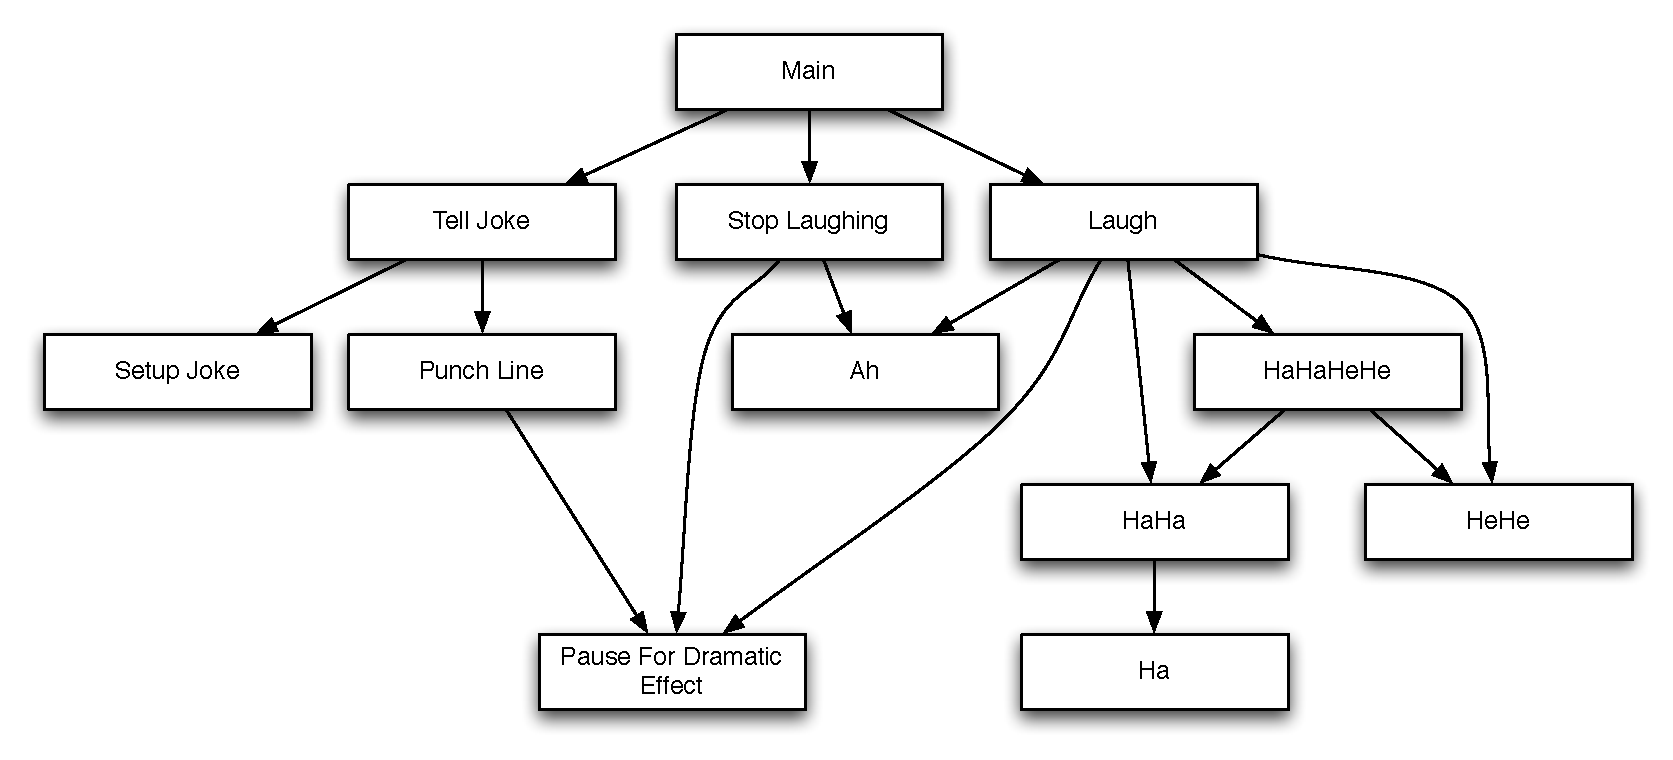
\includegraphics[width=\textwidth]{./topics/procedure-decl/images/TellJokeStructure} 
   \caption{Structure Chart for Tell Joke}
   \label{fig:procedure-decl-tell-joke-struct}
\end{figure}

\csection{The C language does not have a standard \emph{pause} or \emph{delay} procedure, instead of pausing execution the C version will just print ".. pause .." to the Terminal.}

\passection{In Pascal you can use the \texttt{CRT} unit to access a \texttt{Delay} procedure that pauses execution.}

\begin{figure}[p]
   \centering
   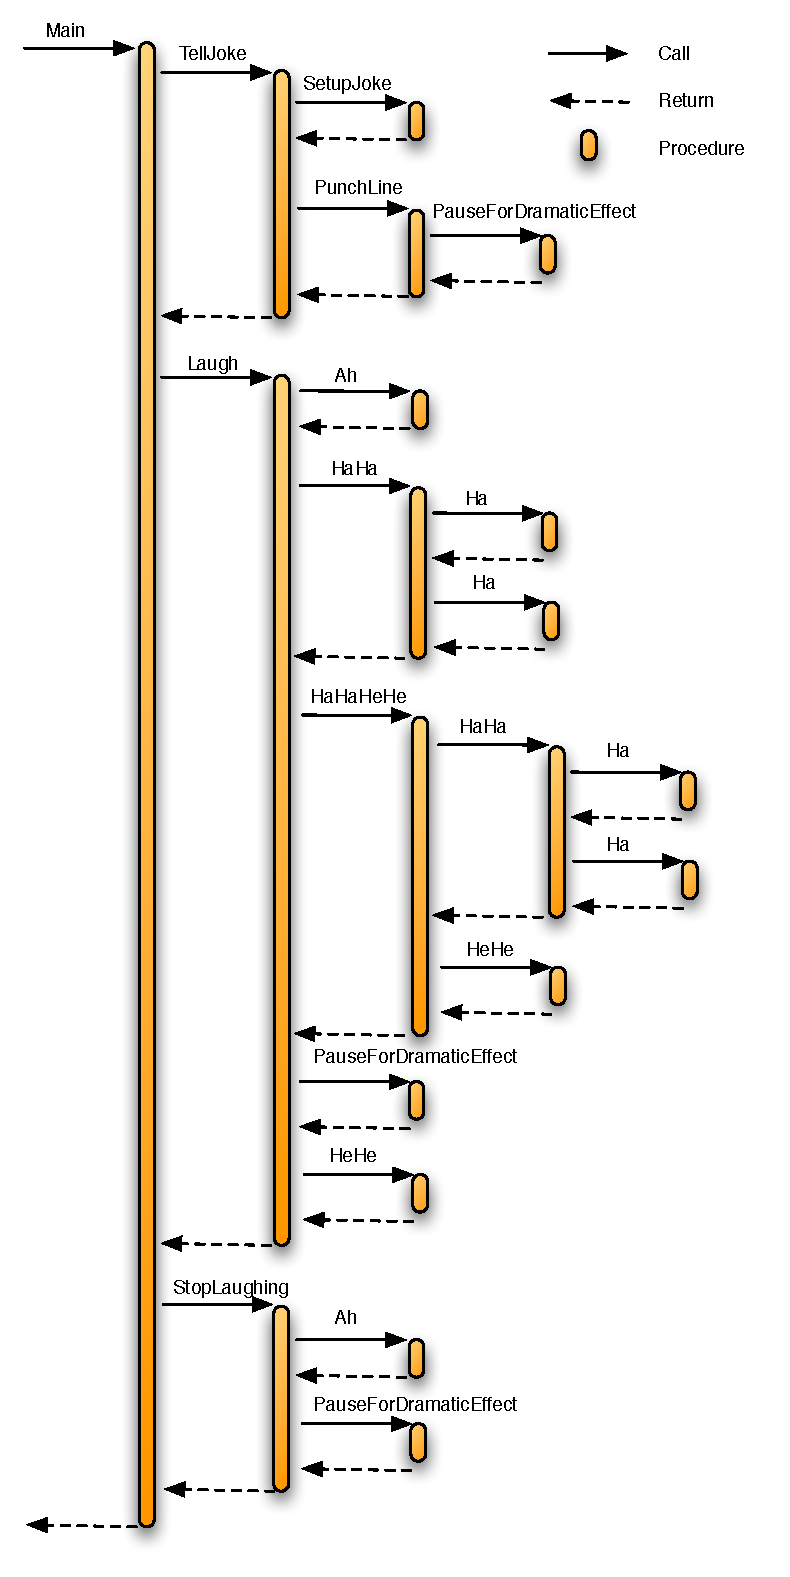
\includegraphics[width=0.7\textwidth]{./topics/procedure-decl/images/TellJokeSeq} 
   \caption{Sequence Diagram for Tell Joke}
   \label{fig:procedure-decl-tell-joke-seq}
\end{figure}


\lpseudocode{lst:procedure-decl-joke-pseudo}{Pseudocode for Tell Joke program.}{./topics/procedure-decl/examples/TellJoke.txt}{2}

\lcsection{\mccode{lst:procedure-decl-tell-joke-c}{C Knock Knock Joke}{topics/procedure-decl/examples/tell-joke.c}{2}}

\lpassection{\mpascode{lst:procedure-decl-tell-joke-pas}{Pascal Knock Knock Joke}{topics/procedure-decl/examples/TellJoke.pas}{2}}


% subsection knock_knock (end)

\subsection{Audio Morse Code} % (fold)
\label{sub:audio_morse_code}

This Chapter explained the development of a \emph{Morse Calling} program that output text to the Terminal. This version of the program uses \textbf{SwinGame} to play audio for the \emph{long} and \emph{short} signals.
\begin{itemize}
  \item The description of the program is in Table \ref{tbl:procedure-decl-morse-audio}
  \item The pseudocode is in Listing \ref{lst:procedure-decl-morse-audio-pseudo}
  \item The Structure Chart is very similar to the version that wrote its output to the Terminal, see Figure \ref{fig:procedure-decl-morsecalling-structure}. This code also include a \texttt{LoadSounds} procedure called from \texttt{Main}.
  \item The dynamic behaviour is the same as the the Sequence Diagram in Figure \ref{fig:procedure-decl-morsecalling-sequence}
  \item Listing \ref{lst:procedure-morse-calling-audio-c} has the C code for the Program
  \item Listing \ref{lst:procedure-morse-calling-audio-pas} has the Pascal code for the Program
\end{itemize}

\begin{table}[h]
\centering
\begin{tabular}{l|p{10cm}}
  \hline
  \multicolumn{2}{c}{\textbf{Program Description}} \\
  \hline
  \textbf{Name} & \emph{Morse Calling} \\
  \\
  \textbf{Description} & Plays audio for the morse code of `\emph{Calling Anyone}'. \\
  \hline
\end{tabular}
\caption{Description of the Morse Calling program}
\label{tbl:procedure-decl-morse-audio}
\end{table}

\csection{
\emph{SwinGame} has the following procedures that can help you implement this program:
\begin{itemize}
  \item \texttt{\textbf{play\_sound\_effect}}: you pass it the name of the sound effect to play.
  \item \texttt{\textbf{delay}}: allows you to pause execution for a number of milliseconds.
  \item \texttt{\textbf{load\_sound\_effect\_named}}: you pass it the name to use, and the filename to load. SwinGame will load the file from \emph{Resources/Sounds}.
  \item \texttt{\textbf{open\_audio}}: starts SwinGame's audio system, you cannot load or play sounds until after this is called.
  \item \texttt{\textbf{close\_audio}}: closes SwinGame's audio system, needed at the end of the program to match the \texttt{open\_audio}.
  \item \texttt{\textbf{release\_all\_resources}}: releases the loaded sound effects.
\end{itemize}
}

\passection{
\emph{SwinGame} has the following procedures that can help you implement this program:
\begin{itemize}
  \item \texttt{\textbf{PlaySoundEffect}}: you pass it the name of the sound effect to play.
  \item \texttt{\textbf{Delay}}: allows you to pause execution for a number of milliseconds.
  \item \texttt{\textbf{LoadSoundEffectNamed}}: you pass it the name to use, and the filename to load. SwinGame will load the file from \emph{Resources/Sounds}.
  \item \texttt{\textbf{OpenAudio}}: starts SwinGame's audio system, you cannot load or play sounds until after this is called.
  \item \texttt{\textbf{CloseAudio}}: closes SwinGame's audio system, needed at the end of the program to match the \texttt{OpenAudio}.
  \item \texttt{\textbf{ReleaseAllResources}}: releases the loaded sound effects.
\end{itemize}
}

\clearpage
\pseudocode{lst:procedure-decl-morse-audio-pseudo}{Pseudocode for Morse Calling with Audio.}{./topics/procedure-decl/examples/MorseCalling.txt}


\clearpage
\csection{\ccode{lst:procedure-morse-calling-audio-c}{C Audio Version of Morse Calling}{topics/procedure-decl/examples/morse-calling.c}}

\passection{\pascode{lst:procedure-morse-calling-audio-pas}{Pascal Audio Version of Morse Calling}{topics/procedure-decl/examples/MorseCalling.pas}}


% subsection audio_morse_code (end)
\clearpage
\subsection{Draw Sun Scene} % (fold)
\label{sub:draw_sun}

This small \textbf{SwinGame} creates a procedure to draw a sun in the top left corner of the screen.
\begin{itemize}
  \item The description of the program is in Table \ref{tbl:procedure-decl-draw-sun}
  \item The pseudocode is in Listing \ref{lst:procedure-decl-draw-sun-pseudo}
  \item Listing \ref{lst:procedure-draw-sun-c} has the C code for the Program
  \item Listing \ref{lst:procedure-draw-sun-pas} has the Pascal code for the Program
\end{itemize}

\begin{table}[h]
\centering
\begin{tabular}{l|p{10cm}}
  \hline
  \multicolumn{2}{c}{\textbf{Program Description}} \\
  \hline
  \textbf{Name} & \emph{Morse Calling} \\
  \\
  \textbf{Description} & Draws a simple scene where a sun is drawn in the upper left corner of the screen. \\
  \hline
\end{tabular}
\caption{Description of the Draw Sun Scene program}
\label{tbl:procedure-decl-draw-sun}
\end{table}

\csection{
\emph{SwinGame} has the following procedures that can help you implement this program:
\begin{itemize}
  \item \texttt{\textbf{open\_graphics\_window}}: you pass it the title of the window, and a width and height in pixels.
  \item \texttt{\textbf{delay}}: allows you to pause execution for a number of milliseconds.
  \item \texttt{\textbf{load\_sound\_effect\_named}}: you pass it the name to use, and the filename to load. SwinGame will load the file from \emph{Resources/Sounds}.
  \item \texttt{\textbf{clear\_screen\_to}}: clears the screen to the indicated color.
  \item \texttt{\textbf{refresh\_screen}}: displays the screen. All SwinGame drawing is performed in the background, this displays the screen to the user.
  \item \texttt{\textbf{draw\_circle}} and \texttt{\textbf{fill\_circle}}: draws the outline or fills a circle on the screen. This is passed the color of the circle, its x and y locations, and its radius.
  \item \texttt{\textbf{draw\_line}}: draws a line from one point to another. This is passed the color of the line, the x and y coordinates of the start point, and the x and y coordinates of the end point.
  \item \texttt{\textbf{release\_all\_resources}}: releases the loaded sound effects.
\end{itemize}
}

\passection{
\emph{SwinGame} has the following procedures that can help you implement this program:
\begin{itemize}
  \item \texttt{\textbf{OpenGraphicsWindow}}: you pass it the title of the window, and a width and height in pixels.
  \item \texttt{\textbf{Delay}}: allows you to pause execution for a number of milliseconds.
  \item \texttt{\textbf{ClearScreen}}: clears the screen to the indicated color.
  \item \texttt{\textbf{RefreshScreen}}: displays the screen. All SwinGame drawing is performed in the background, this displays the screen to the user.
  \item \texttt{\textbf{DrawCircle}} and \texttt{\textbf{FillCircle}}: draws the outline or fills a circle on the screen. This is passed the color of the circle, its x and y locations, and its radius.
  \item \texttt{\textbf{DrawLine}}: draws a line from one point to another. This is passed the color of the line, the x and y coordinates of the start point, and the x and y coordinates of the end point.
  \item \texttt{\textbf{ReleaseAllResources}}: releases the loaded sound effects.
\end{itemize}
}

\mynote{
SwinGame colors are \texttt{ColorBlue, ColorGreen, ColorRed, ColorWhite, ColorBlack, ColorYellow,
ColorPink, ColorTurquoise, ColorGrey, ColorMagenta, and ColorLightGrey}.
}


\clearpage
\pseudocode{lst:procedure-decl-draw-sun-pseudo}{Pseudocode for Draw Sun Scene program}{./topics/procedure-decl/examples/draw-sun.txt}


\clearpage
\csection{\ccode{lst:procedure-draw-sun-c}{C Draw Sun Scene Program}{topics/procedure-decl/examples/draw-sun.c}}

\passection{\pascode{lst:procedure-draw-sun-pas}{Pascal Draw Sun Scene Program}{topics/procedure-decl/examples/DrawSun.pas}}



% subsection draw_sun (end)
